\documentclass[a4paper, 11pt, oneside]{article}

\usepackage[utf8]{inputenc}
\usepackage[T1]{fontenc}
\usepackage[french]{babel}
\usepackage{array}
\usepackage{shortvrb}
\usepackage{listings}
\usepackage[fleqn]{amsmath}
\usepackage{amsfonts}
\usepackage{fullpage}
\usepackage{enumerate}
\usepackage{graphicx}
\usepackage{subfigure}
\usepackage{alltt}
\usepackage{url}
\usepackage{indentfirst}
\usepackage{eurosym}
\usepackage{listings}
\usepackage{titlesec, blindtext, color}
\usepackage[table,xcdraw,dvipsnames]{xcolor}
\usepackage[unicode]{hyperref}
\usepackage{url}
\usepackage{float}

\definecolor{mygray}{rgb}{0.5,0.5,0.5}

\lstset{
    language=C, % Utilisation du langage C
    commentstyle={\color{MidnightBlue}}, % Couleur des commentaires
    frame=single, % Entoure le code d'un joli cadre
    rulecolor=\color{black}, % Couleur de la ligne qui forme le cadre
    stringstyle=\color{RawSienna}, % Couleur des chaines de caractères
    numbers=left, % Ajoute une numérotation des lignes à gauche
    numbersep=5pt, % Distance entre les numérots de lignes et le code
    numberstyle=\tiny\color{mygray}, % Couleur des numéros de lignes
    basicstyle=\tt\footnotesize, 
    tabsize=3, % Largeur des tabulations par défaut
    keywordstyle=\tt\bf\footnotesize\color{Sepia}, % Style des mots-clés
    extendedchars=true, 
    captionpos=b, % sets the caption-position to bottom
    texcl=true, % Commentaires sur une ligne interprétés en Latex
    showstringspaces=false, % Ne montre pas les espace dans les chaines de caractères
    escapeinside={(>}{<)}, % Permet de mettre du latex entre des <( et )>.
    inputencoding=utf8,
    literate=
  {á}{{\'a}}1 {é}{{\'e}}1 {í}{{\'i}}1 {ó}{{\'o}}1 {ú}{{\'u}}1
  {Á}{{\'A}}1 {É}{{\'E}}1 {Í}{{\'I}}1 {Ó}{{\'O}}1 {Ú}{{\'U}}1
  {à}{{\`a}}1 {è}{{\`e}}1 {ì}{{\`i}}1 {ò}{{\`o}}1 {ù}{{\`u}}1
  {À}{{\`A}}1 {È}{{\`E}}1 {Ì}{{\`I}}1 {Ò}{{\`O}}1 {Ù}{{\`U}}1
  {ä}{{\"a}}1 {ë}{{\"e}}1 {ï}{{\"i}}1 {ö}{{\"o}}1 {ü}{{\"u}}1
  {Ä}{{\"A}}1 {Ë}{{\"E}}1 {Ï}{{\"I}}1 {Ö}{{\"O}}1 {Ü}{{\"U}}1
  {â}{{\^a}}1 {ê}{{\^e}}1 {î}{{\^i}}1 {ô}{{\^o}}1 {û}{{\^u}}1
  {Â}{{\^A}}1 {Ê}{{\^E}}1 {Î}{{\^I}}1 {Ô}{{\^O}}1 {Û}{{\^U}}1
  {œ}{{\oe}}1 {Œ}{{\OE}}1 {æ}{{\ae}}1 {Æ}{{\AE}}1 {ß}{{\ss}}1
  {ű}{{\H{u}}}1 {Ű}{{\H{U}}}1 {ő}{{\H{o}}}1 {Ő}{{\H{O}}}1
  {ç}{{\c c}}1 {Ç}{{\c C}}1 {ø}{{\o}}1 {å}{{\r a}}1 {Å}{{\r A}}1
  {€}{{\euro}}1 {£}{{\pounds}}1 {«}{{\guillemotleft}}1
  {»}{{\guillemotright}}1 {ñ}{{\~n}}1 {Ñ}{{\~N}}1 {¿}{{?`}}1
}

%%%% Page de garde %%%%

\title{Codage de Prüfer}
\author{Maxime GOFFART - Olivier JORIS}
\date{2019 - 2020}

\begin{document}

\maketitle
\newpage

\tableofcontents
\newpage

\section{Introduction}

\paragraph{}
Le codage de Prüfer permet d'encoder un arbre composé de n sommets (avec des labels différents compris entre 1 et n) via une suite de n - 2 naturels. Il existe donc une bijection entre un arbre dont les n sommets sont numérotés et son codage de Prüfer, ce qui implique qu'un seul arbre admet un seul codage de Prüfer et inversement.\\
Cette bijection permet de facilement démontrer la formule de Cayley:\\
\textit{Soit n > 1, on peut construire exactement $n^{n-2}$ arbres différents constitués de n sommets.}

\begin{figure}[H]
	\centering
	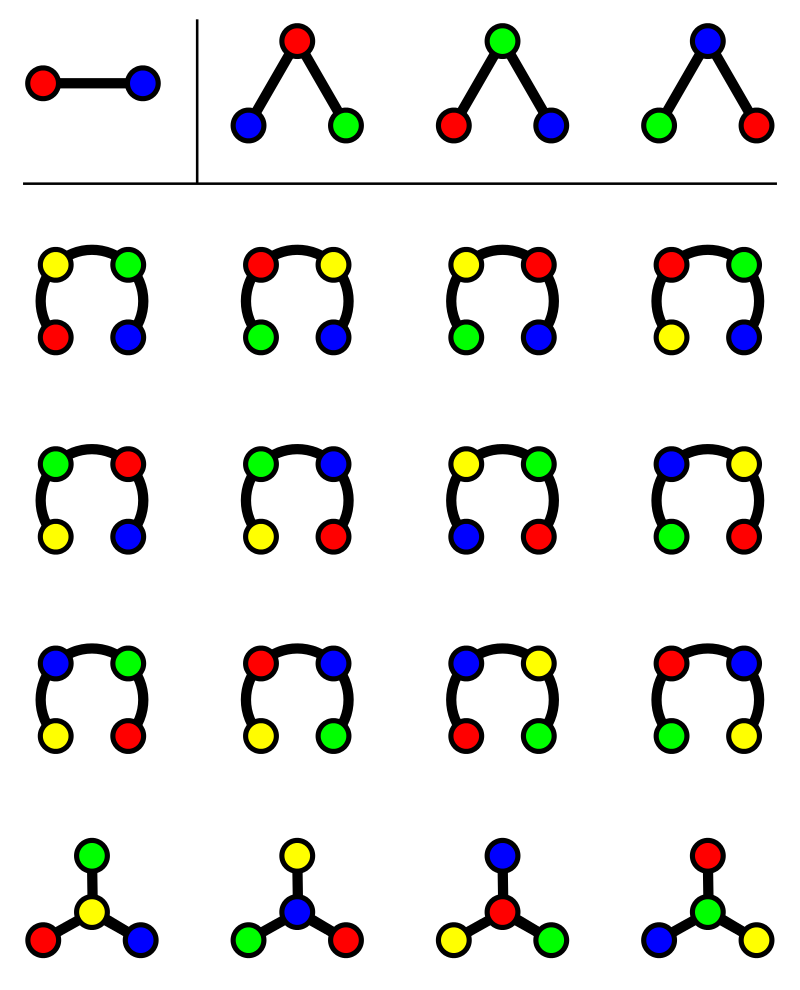
\includegraphics[scale=0.2]{formule_Cayley.png} 
	\caption{Liste complète des arbres à 2, 3 et 4 sommets\protect\footnotemark}
\end{figure}

\footnotetext{Source : \url{https://fr.wikipedia.org/wiki/Formule_de_Cayley}}

Ce codage permet également de représenter un arbre sans utiliser sa matrice d'adjacence ou sa liste d'adjacence. De cela découle une optimisation de sa complexité spatiale et par conséquent des complexités temporelles des algorithmes le manipulant.\\

Nous avons réalisé un programme qui, à un arbre donné, donne son codage de Prüfer et inversement.

\section{Mode d'emploi du programme}

Le programme peut être compilé à l'aide du \textit{makefile} via la commande suivante:

\begin{lstlisting}[language=bash]
$ make prufer
\end{lstlisting}

Un exécutable nommé \texttt{prufer} est alors créé, celui-ci peut être lancé à l'aide de deux arguments:

\begin{lstlisting}[language=bash]
$ ./prufer -m encodage -f exempleGraphe.txt
\end{lstlisting}

où l'option \texttt{-m} désigne le mode d'utilisation du programme\footnote{encodage ou decodage}. L'option \texttt{-f} désigne le fichier contenant la matrice d'adjacence du graphe en cas d'encodage et la suite de Prüfer (précédée de sa longueur sur la première ligne) en cas de décodage. Des exemples de fichiers sont disponibles dans le dossier \texttt{/code}.

\section{Stratégie adoptée}

Le codage de Prüfer s'appliquant uniquement aux arbres, nous avons d'abord implémenté des fonctions vérifiant que le graphe fourni par l'utilisateur soit un arbre\footnote{En cas d'encodage}.

Ensuite, nous nous sommes renseignés sur le fonctionnement des algorithmes d'encodage et de décodage (via ce lien: \url{https://fr.wikipedia.org/wiki/Codage_de_Pr%C3%BCfer}) et nous les avons implémentés.

\section{Choix opérés}

Nous avons choisi de représenter un codage de Prüfer grâce à la structure suivante, permettant de directement accéder à la taille de la séquence de nombres: 

\begin{lstlisting}
typedef struct CodagePrufer_t{
	unsigned int taille; // La taille du codage de Prüfer
	int* suitePrufer; // La suite de Prüfer (suite de nombres)
}CodagePrufer;
\end{lstlisting}

En ce qui concerne la représentation des graphes, nous avons choisi d'utiliser l'interface \texttt{graphes.c/graphes.h} qui nous était proposée en y ajoutant différentes fonctions.

\section{Principales fonctions}

Les principales fonctions composant notre programme sont:\\

\begin{itemize}

\item[\textbullet] Des fonctions vérifiant si le graphe est un arbre:\\

\begin{itemize}

	\item[-] \texttt{test\_connexite}: Vérifie si un graphe donné en argument est connexe.
	
	\item[-] \texttt{est\_non\_oriente}: Vérifie si un graphe donné en argument est non orienté.

	\item[-] \texttt{contient\_cycle}: Vérifie si un graphe donné en argument contient au moins un cycle.\\

\end{itemize}

\item[\textbullet] Des fonctions d'encodage d'un graphe et de décodage d'une séquence de Prüfer:\\

\begin{itemize}

	\item[-] \texttt{generer\_codage\_prufer}: Génère le codage associé à l'arbre donné.
	
	\item[-] \texttt{decoder\_codage\_prufer}: Génère l'arbre associé au codage de Prüfer donné.

\end{itemize}

\end{itemize}

\section{Difficultés rencontrées}

Les principales difficultés rencontrées étaient liées aux manipulations de liste d'adjacence du graphe donné. Un schéma représentant celle-ci facilite leur manipulation.

\section{Résultats expérimentaux}

Les résultats suivants ont été obtenus en mesurant empiriquement les temps de calcul des fonctions d'encodage d'un arbre et de décodage d'une suite de Prüfer. Ceux-ci ont été obtenus en générant aléatoirement une suite de Prüfer qui a ensuite été décodée puis, grâce au graphe résultant, a été encodée. Les fonctions prévues à cet effet sont situées dans le module \texttt{prufer\_benchmarking.c}. Ce module peut être compilé séparément du programme principal grâce à l'utilisation de la commande suivante:

\begin{lstlisting}[language=bash]
$ make prufer_benchmarking 
\end{lstlisting}

Un exécutable \texttt{prufer\_benchmarking} est alors créé, celui-ci peut-être lancé à l'aide d'un argument désignant le nombre de sommets composant l'arbre généré aléatoirement:

\begin{lstlisting}[language=bash]
$ ./prufer_benchmarking 1000
\end{lstlisting}

Une fois le temps de calcul écoulé, celui-ci est disponible avec le nombre de sommet correspondant sur une nouvelle ligne des fichiers \texttt{resultats\_encodage.txt} pour le temps d'encodage et \texttt{resultats\_decodage.txt} pour le temps de décodage.\\

Ces tests ont été effectués sur une machine dotée d'un Intel Core i5 de 2 coeurs cadencés à 2.3 GHz. Le code a été compilé avec l'optimisation au niveau\footnote{L'option \texttt{-O3} de \texttt{GCC}.} 3.

\begin{figure}[H]
	\centering
	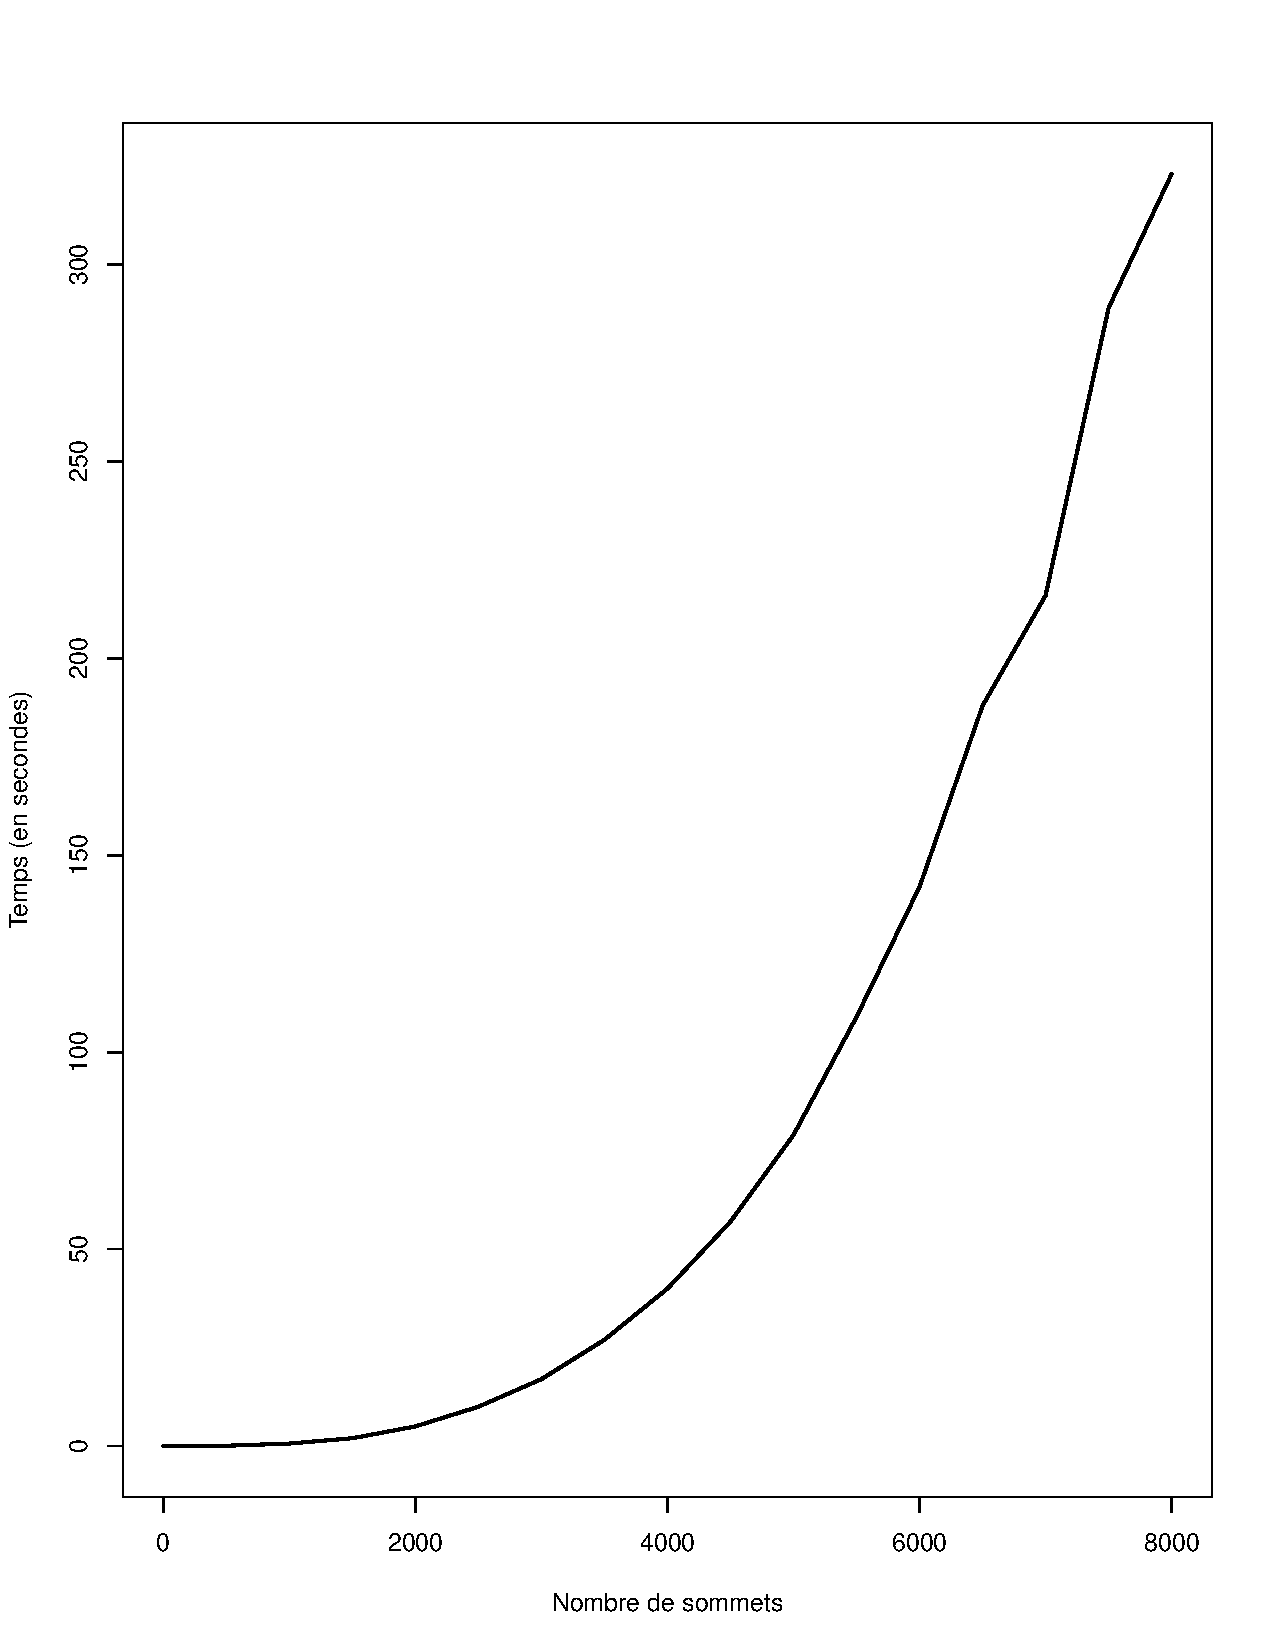
\includegraphics[scale=0.5]{temps_encodage.pdf} 
	\caption{Temps d'encodage en fonction du nombre de sommets de l'arbre}
\end{figure}

\begin{figure}[H]
	\centering
	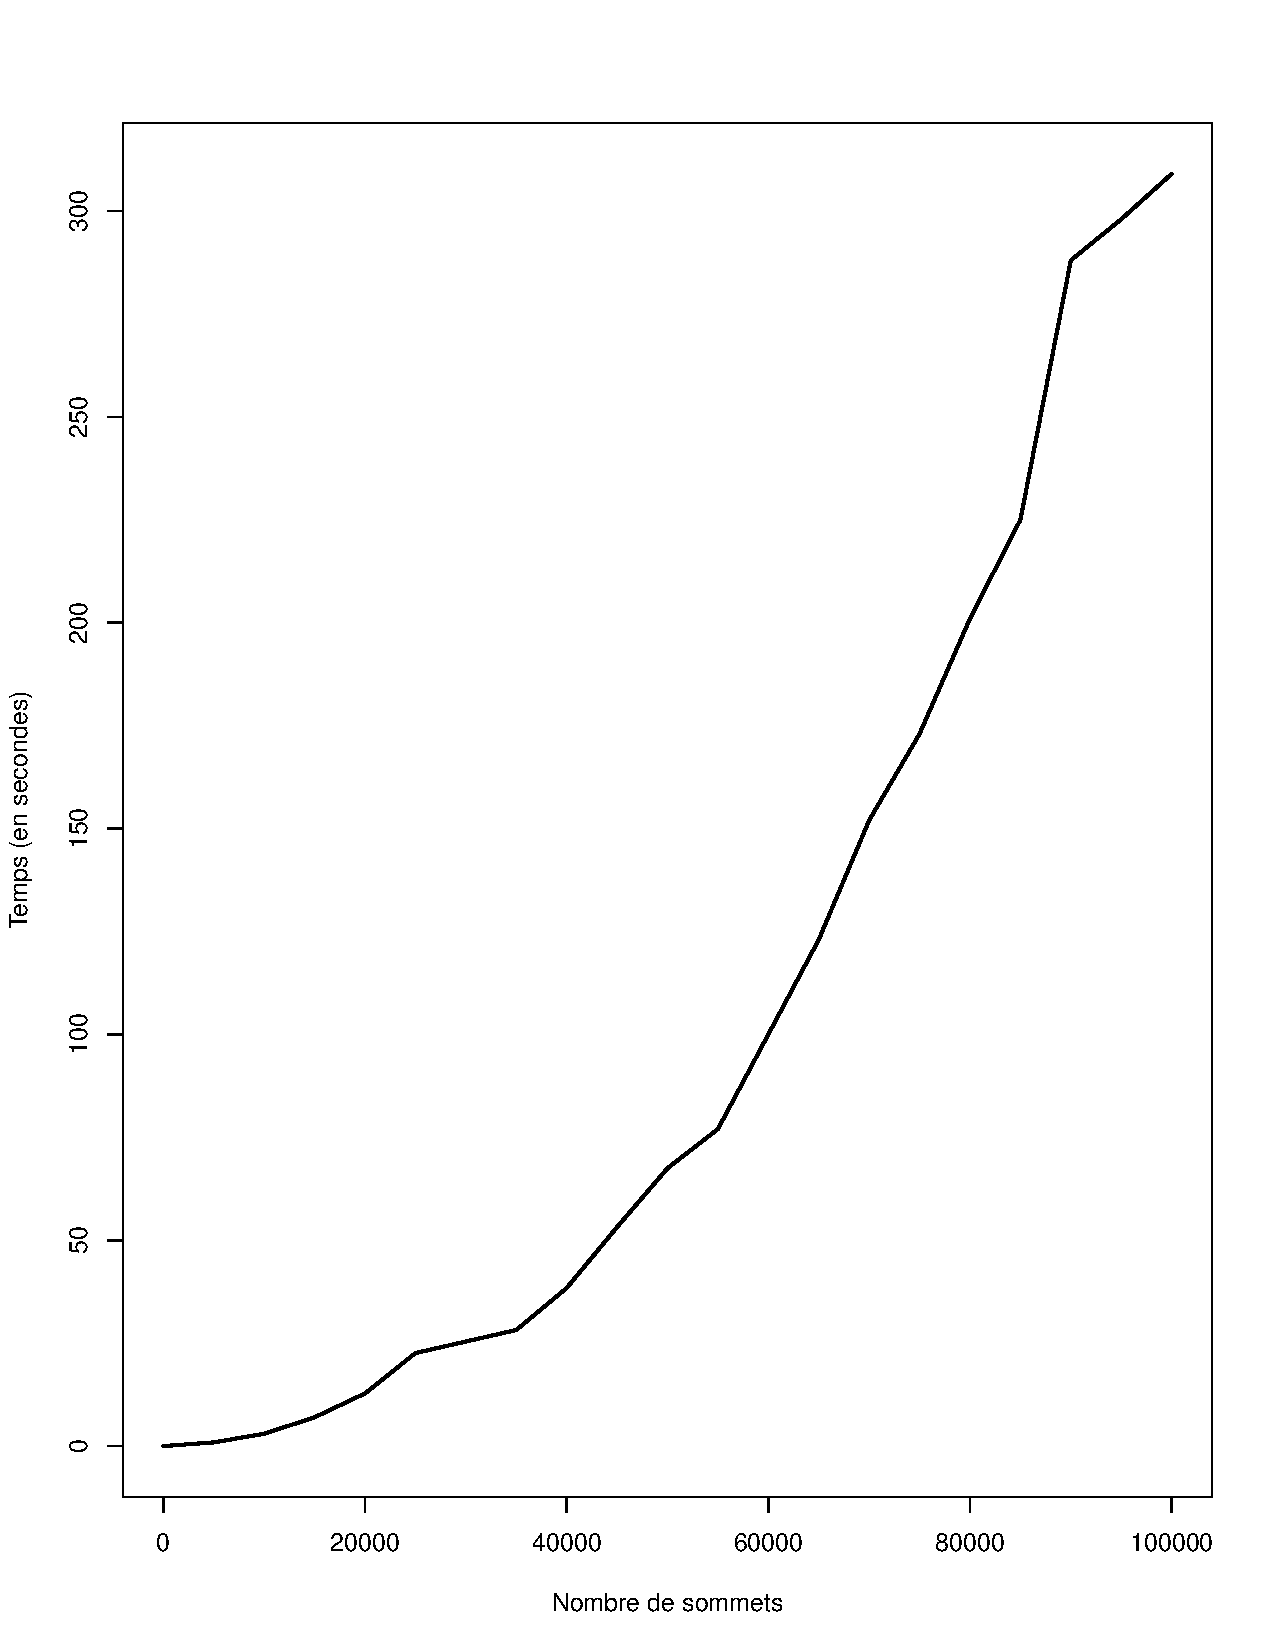
\includegraphics[scale=0.5]{temps_decodage.pdf} 
	\caption{Temps de décodage en fonction du nombre de sommets de l'arbre}
\end{figure}

Sur base des figure 2 et 3, on voit que le temps d'encodage est nettement plus élevé que le temps de décodage. En effet, contrairement au décodage, l'encodage nécessite de rechercher la feuille ayant le plus petit label, ce qui est gourmand en temps.

\end{document}
